% \documentclass[10pt,twoside]{article}
\documentclass{pginz}

\usepackage[utf8]{inputenc}
\usepackage{nicefrac}       % compact symbols for 1/2, etc.
\usepackage{microtype}      % microtypography
\usepackage{ragged2e}
\justifying
\usepackage{float}
\renewcommand{\figurename}{Rysunek}
\usepackage{natbib}
\usepackage{graphicx}
\usepackage{amsmath}
\usepackage{adjustbox}
\usepackage{polski}
\usepackage{gensymb}
\setcitestyle{square}
\usepackage{setspace}
\usepackage{pdfpages}
\usepackage{titlesec}
\usepackage{svg}



\providecommand{\keywordspl}[1]
{
  \small	
  \textbf{\textit{Słowa kluczowe:}} #1
} 
\providecommand{\keywordseng}[1]
{
  \small	
  \textbf{\textit{Keywords:}} #1 
}
\providecommand{\dnauki}[1]
{
  \small	
  \textbf{\textit{Dziedzina nauki i techniki, zgodnie z wymogami OECD:}} #1
}


\begin{document}

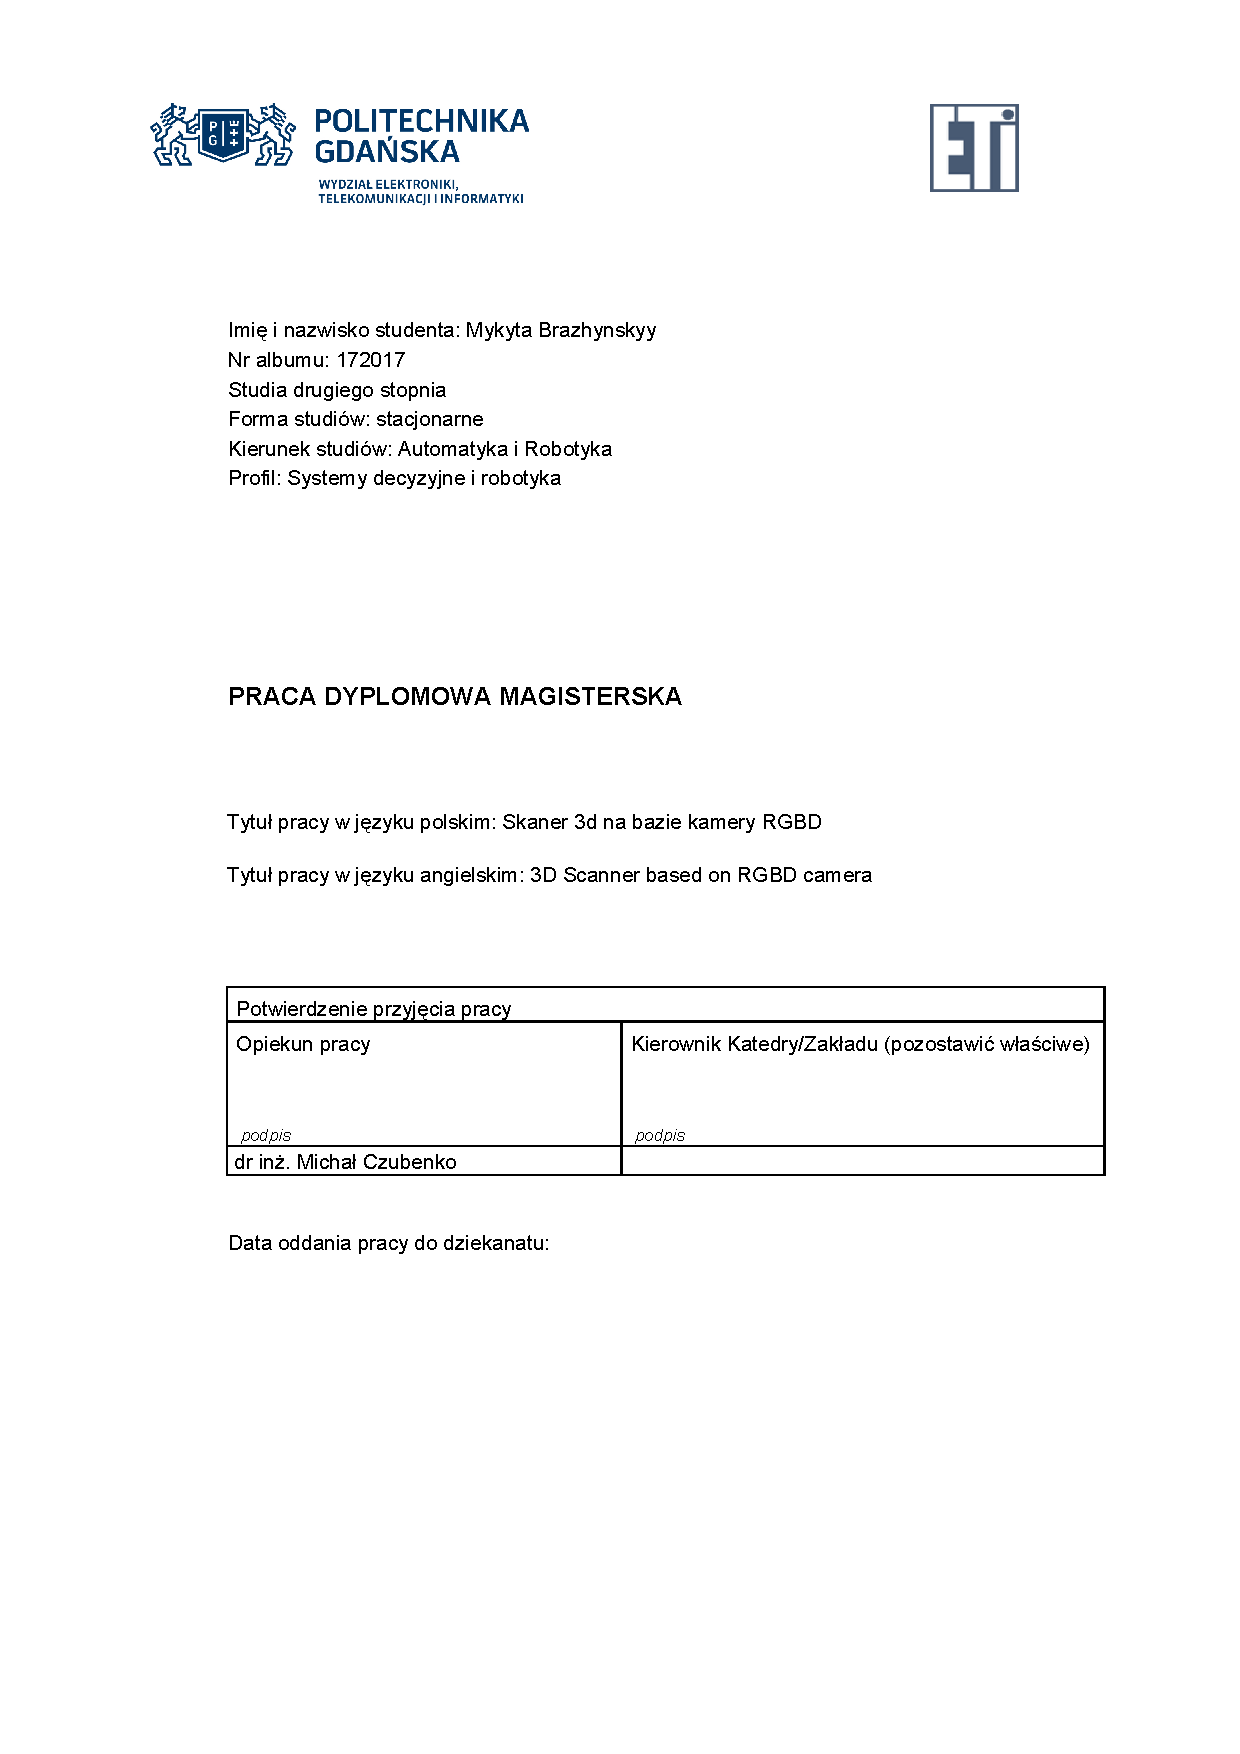
\includepdf[pages=-]{tytolowanowa.pdf}
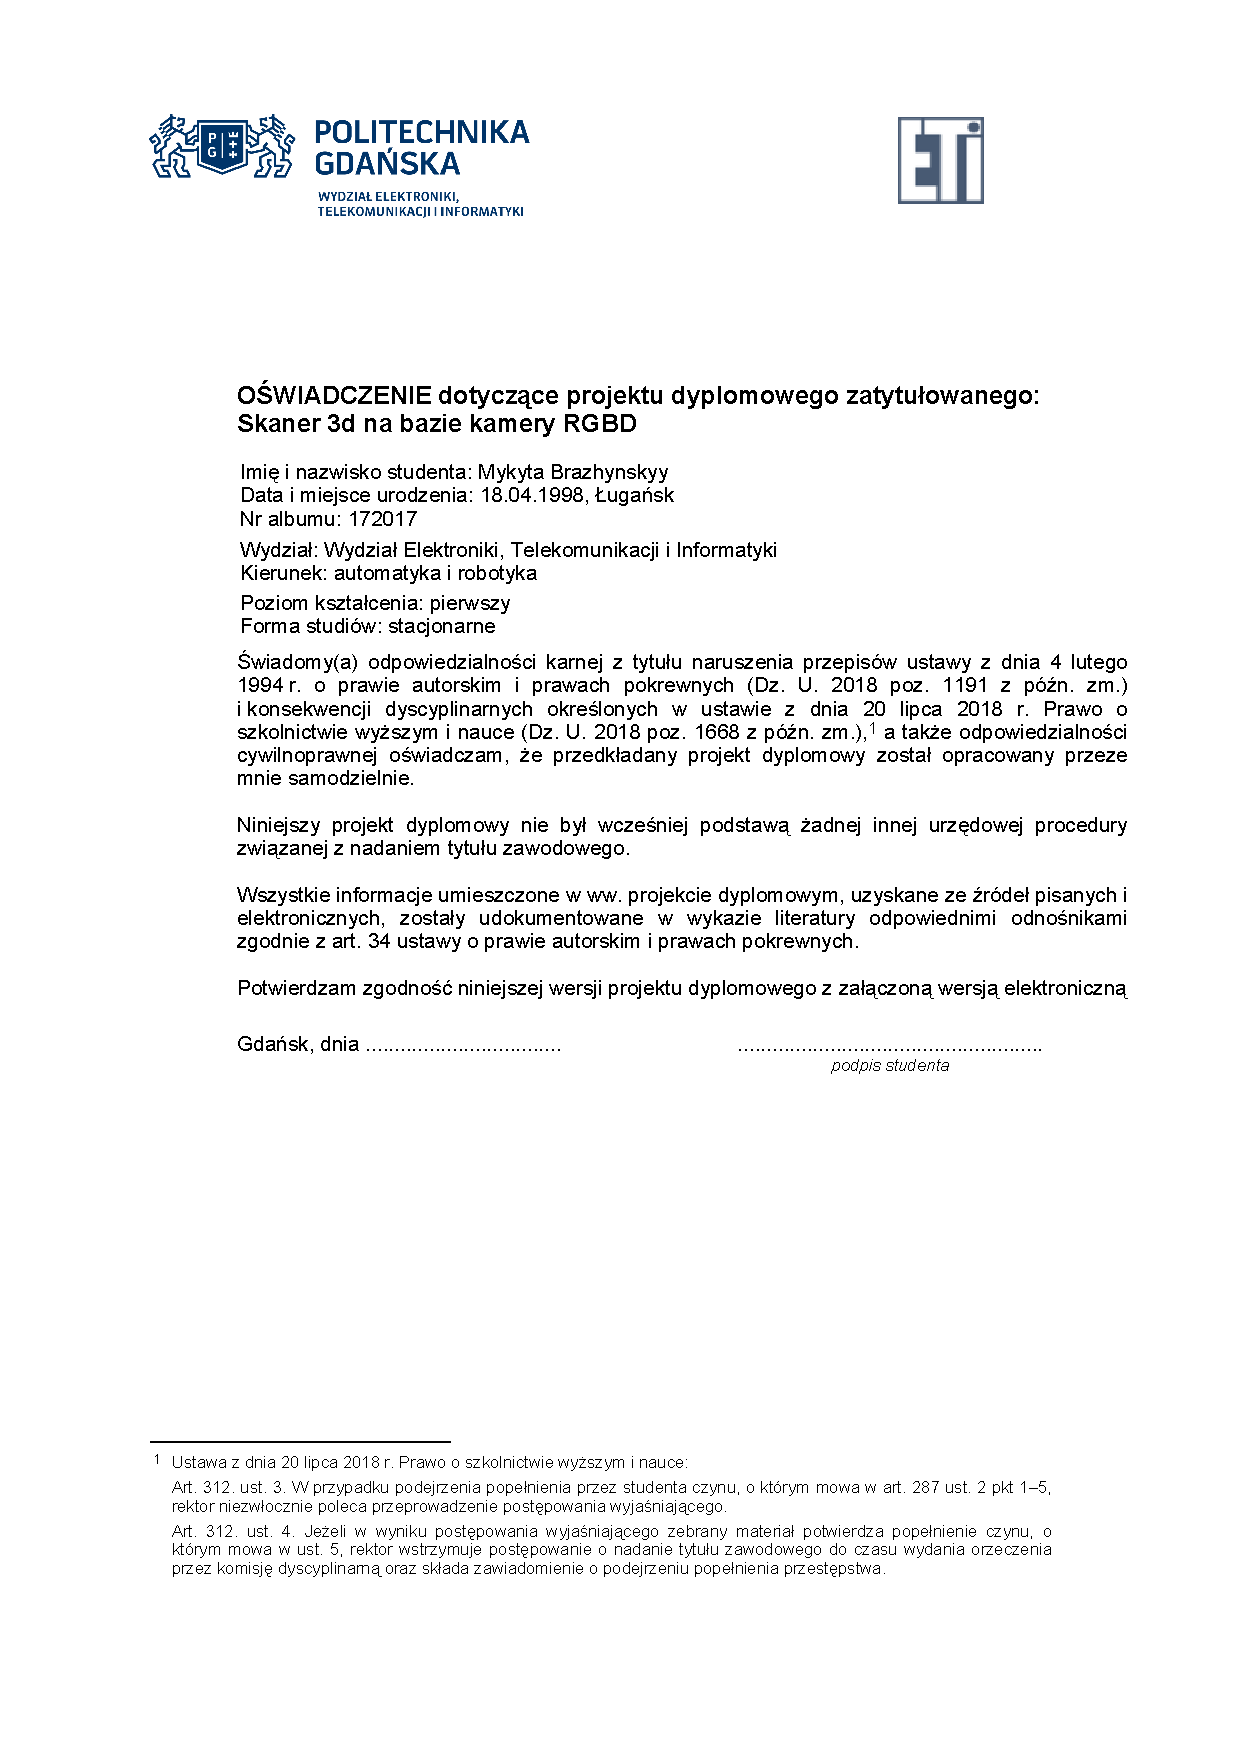
\includepdf[pages=-]{oswiadczenie.pdf}


\setcounter{page}{3}

 
\section*{STRESZCZENIE}
Celem niniejszej pracy dyplomowej było stworzenie skanera 3D oraz systemu wizualizacji utworzonych modeli rzeczywistych obiektów. Do budowy urządzenia wykorzystano kamerę głębi firmy Intel o nazwie RealSense D435i. W pracy został przedstawiony sposób budowy skanera 3D, jego kalibracji oraz algorytmy służące do przetwarzania otrzymanych danych pomiarowych w celu uzyskania wirtualnych modeli. W celu łatwiejszej obsługi programu został utworzony interfejs graficzny zawierający najważniejsze parametry wizualizacji i obróbki danych. Na koniec dane są eksportowane do modeli w formacie obsługiwanym przez program Blender.

\keywordspl{Skaner 3D ,Intel RealSense, Python, Kamera RGBD}

\dnauki{Nauki inżynieryjne i techniczne, Systemy automatyzacji i kontroli }

\section*{ABSTRACT}
The aim of this thesis was to create a 3D scanner and a system for visualization of created models based on real objects. In the work is presented how to build a 3D scanner, its calibration and algorithms used to process the obtained measurement data to obtain virtual models. In order to make the program easier to use, a graphic interface was created containing the most important parameters of visualization and data processing. Finally, the data are exported to the models in a format supported by the Blender program.

\keywordseng{3D Scanner, Intel RealSense, Python, RGBD Camera}
\newpage
\tableofcontents


\newpage

\chapter*{WYKAZ WAŻNIEJSZYCH OZNACZEŃ I SKRÓTÓW}
\subsection*{RGB}
Paleta barw tworząca kolor piksela. Oznaczenie pochodzi od kolorów Red, Green, Blue czyli czerwony, zielony, niebieski.
\subsection*{Kamera RGBD}
Kamera głębi, oprócz wykonywania zdjęć RGB potrafi ona również dokonać pomiaru odległości od obiektów i nanieść te informację na powierzchnię poszczególnych pikseli obrazu.
\subsection*{LIDAR}
Ang.(Light Detection And Ranging) urządzenie służące do dokładnego pomiaru odległości. Działaniem przypomina funkcjonowanie radaru, lecz korzysta z odliczania czasu przelotu światła lasera, a nie mikrofal.
\subsection*{Blender}
Oprogramowanie służące do modelowania trójwymiarowego.Posiada szereg funkcji do animacji obiektów, generacji tekstur oraz importowania i eksportowania gotowych modeli.
\subsection*{Maya}
Program komputerowy, umożliwiający generację zaawansowanych modeli 3D przeznaczony do zastosowań przemysłowych. W tym programie zostały stworzone filmy takie jak Spiderman, Avatar oraz Up.
\subsection*{LIDAR}
Skaner impulsowy LIDAR jest urządzeniem mierzącym odległość za pomocą wiązki światła. Jego zasada działania jest zbliżona do funkcjonowania radaru.
\chapter{WSTĘP I CEL PRACY}
\section{Wprowadzenie}
W bieżącym rozdziale przedstawione zostaną wyniki implementacji dwóch metod rekonstrukcji powierzchni z chmury punktów. Omówione zostaną charakterystyki poszczególnych algorytmów oraz rezultaty dzięki nim uzyskane. Ukazana zostanie implementacja wybranego z nich.
W celu uzyskania trójwymiarowych modeli na podstawie skanów rzeczywistych obiektów, przetestowano dwie metody generacji meshu. Pierwszą z nich jest ball pivoting algorithm. Kolejnym algorytmem będzie trójwymiarowa triangulacja Delaunay'a.


\section{Cele i założenia}
Celem niniejszej pracy jest zaprojektowanie skanera 3D korzystającego z metody triangulacji laserowej  oraz wyeksportowanie modeli do programu Blender przy zastosowaniu kamery RGBD. Projekt składa się z dwóch części, budowy skanera trójwymiarowego oraz stworzenie programu do obróbki otrzymanych danych. Odległość z jakiej będzie wykonywany skan wynosi do 1 m. Powyżej tej wartości gęstość punktów będzie zbyt niska do wiernego odtworzenia modelu. Czas trwania obliczeń w programie wynosi poniżej 15 minut. Utworzony model powinien jak najwierniej oddawać wygląd rzeczywistego obiektu, luki w teksturze powinny nieznacznie wpływać na ostateczny wygląd.

\section{Zawartość pracy}
Pierwszy rozdział opisuje cele oraz założenia pracy.Dokonano gruntownej analizy problemu, który zostanie rozwiązany w dalszym ciągu pracy.

W drugim rozdziale wykonano przegląd istniejących metod mających na celu generację trójwymiarowych obiektów na podstawie danych z kamery głębi. Dokonano porównania pomiędzy dostępnymi na rynku skanerami 3D bazującymi na różnych technologiach pomiarowych. Wymieniono ich parametry techniczne. Zobrazowano w jakich warunkach dana metoda pomiarowa powinna zostać wykorzystana. Ukazane zostały również technologie jakimi posługiwano się w przeszłości do generacji trójwymiarowych modeli. Na koniec przedstawione zostały zastosowania współczesnych skanerów 3D.

W kolejnym rozdziale przedstawiony jest model oraz konstrukcja skanera 3D. Wyjaśniono metody służące do przetworzenia danych uzyskanych z kamery głębi w chmurę punktów. Przedstawiono koncepcje istniejących rozwiązań służących do rekonstrukcji powierzchni oraz kształtu obiektów z chmury punktów.

Czwarty rozdział przedstawia podsumowanie zarówno wykonanej pracy, jak i otrzymanych efektów. Ukazane zostaną również metody analizy oraz obróbki danych, które mają posłużyć do cyfrowej implementacji rzeczywistych obiektów zarejestrowanych przez kamerę RGBD. Przedstawiono opisy zastosowanych algorytmów oraz kolejność ich wykonywania na podstawie autorskiego programu w języku Python. Poddano analizie pod względem dokładności rezultaty pomiarów w porównaniu do rzeczywistych wartości mierzonych.

Ostatni rozdział porusza kwestię potencjalnych możliwości udoskonalenia urządzenia.

\section{Wprowadzenie}
W bieżącym rozdziale przedstawione zostaną wyniki implementacji dwóch metod rekonstrukcji powierzchni z chmury punktów. Omówione zostaną charakterystyki poszczególnych algorytmów oraz rezultaty dzięki nim uzyskane. Ukazana zostanie implementacja wybranego z nich.
W celu uzyskania trójwymiarowych modeli na podstawie skanów rzeczywistych obiektów, przetestowano dwie metody generacji meshu. Pierwszą z nich jest ball pivoting algorithm. Kolejnym algorytmem będzie trójwymiarowa triangulacja Delaunay'a.






\renewcommand{\listtablename}{Spis tabel}
\renewcommand{\listfigurename}{Spis rysunków}
\addcontentsline{toc}{chapter}{Spis tabel}
\addcontentsline{toc}{chapter}{Spis rysunków}
\listoffigures
\listoftables


\addcontentsline{toc}{chapter}{Bibliografia}
\bibliography{references}
\bibliographystyle{ieeetr}
\end{document}
